\documentclass[main]{subfiles}
\begin{document}

%@@@@@@@@@@@@@@@@@@@@@@@@@@@@@@
% Main Topics: definitions of basis, reduced cost, degeneracy and basic idea of
% simplex algorithm
% Simplex Algorithm I - 16.10.2017
% author:

\section{Simplex Algorithm I}

$A \in \mathbb{Q}^{m \times n}$, $b \in \mathbb{Q}^n$. Consider $\min \{c^T x 
\mid Ax = b$, $x \geq 0 \} (\mathcal{P})$. and $max \{b^T y \mid y^T A \leq c^T 
\}(D)$.

We assume $m < n$ (otherwise, extra rows are linearly dependent, and for $m=n$
we have exact one solution or no solution).

\textbf{Recall:} $B \subseteq \{1, \dots, n \}$ is a basis if $|B| = m$ and
$A_B$ is invertible. $A_B$ submatrix of $A \in \mathbb{R}^{m \times n}$ with
column vectors $A_{\cdot , j}$ for $j \in B$.

\textbf{Notation} For $x \in \mathbb{R}^n$ we write
$x =
\begin{pmatrix}
x_B \\
x_N
\end{pmatrix}$
, where $N = \{1, \dots, n \}\setminus B$, i.e, $N$ is the complement of $B$.

\paragraph{Definition: Given a basis $B$, we define the following points:}
$(y^*)^T = c^T_B A^{-1}_B$ and
$x^* = 
\begin{pmatrix}
x^*_B \\
x^*_N
\end{pmatrix}$ with $x^*_N = 0$, $x^*_B = A^{-1}_B b$

$y^*$ is a dual basic solution (not necessarily feasible), the same way, $x^*$
is a primal basic solution (not necessarily feasible), and they satisfy 
complementary slackness: $\forall i$: $x^*_i (c_i -(y^*_j)^T A_{\cdot j}) = 0$.

\paragraph{Lemma:}
\begin{enumerate}
\item $y^*$ is a dual feasible $\iff \forall j \in N$: $c_j - 
c_B^T A^{-1}_B A_{\cdot j} \geq 0$
\item $x^*$ is a primal feasible $\iff A^{-1}_B b \geq 0$
\end{enumerate}

\subparagraph{Proof:}
\begin{enumerate}
\item $y^*$ is dual feasible $\iff (y^*)^T A \leq c^T \iff \forall j$:
$(y^*)^T A_{\cdot j} \leq c_j \iff \forall j \in N$: $c^T_B A^{-1}_B
A_{\cdot j} \leq c_j \iff \forall j \in N$: $c_j - c^T_B A^{-1}_B A_{\cdot j}
\geq 0$.
\item $Ax^* = A_B x^*_B + A_N \underbrace{x^*_N}_{=0} = A_B x^*_B$,
$x^*$ is primal feasible $\iff x^* \geq 0$ and $\forall i \in N$:
$x_i = 0 \iff 0 \leq x^*_B = A^{-1}_B b$ 
\end{enumerate}

\paragraph{Definition: Reduced cost}
We define the vector of reduced cost $\bar{c} \in \mathbb{R}^{n - m}$ by
$\bar{c_j} = c_j - c^T_B A^{-1}_B A_{\cdot j}$\\
Define $\bar{b} = A^{-1}_B b$\\
Define $\bar{A} = A^{-1}_B A = [\mathcal{I} | A^{-1}_B A_N ]$

The basic idea for an algorithm:\\
\begin{figure}[!h]
  \label{fig:projection}
  \centering
    
\includegraphics[width=0.3\textwidth]{imgs/simplex-description.png}
\end{figure}

Take initial point $x_o \in \mathcal{P}$. While $x_0$ not optimal, determine
direction $d \in \mathbb{R}^n$, $\lambda > 0$ st $c^T d \leq 0$ and
$x_0 + \lambda d \in \mathcal{P}$. Set $x_1 = x_0 + \lambda d$ and iterate.

\textbf{Questions: How do we find an initial point? How to determine $d$ and
$\lambda$ fast? When to stop?}

\subsection{Degeneracy}
\paragraph{Definition:}
\begin{enumerate}
\item For $\mathcal{P} = \{x \in \mathbb{R}^n \mid Ax \leq b\}$ (canonical
form), a bfs $x^*$ is degenerated if $|I(x^*)| > n$, where
$I(x^*) = \{i \in \{1, \dots, m\} \mid A_{i\cdot}x^* = b_i\}$, i.e, more than
$n$ constraints are tight.
\item For $\mathcal{P} = \{x \in \mathbb{R}^n_+ \mid Ax = b\}$ (standard form),
a bfs $x^*$ is degenerated if more than $n-m$ components of $x^*$ are equal to
zero, i.e, some entries of $x^*_B$ are zero.
\end{enumerate}

There are differents ways such that degeneracy arises.\\
Examples:\\

(i)\\
\begin{figure}[!h]
  \label{fig:projection}
  \centering
    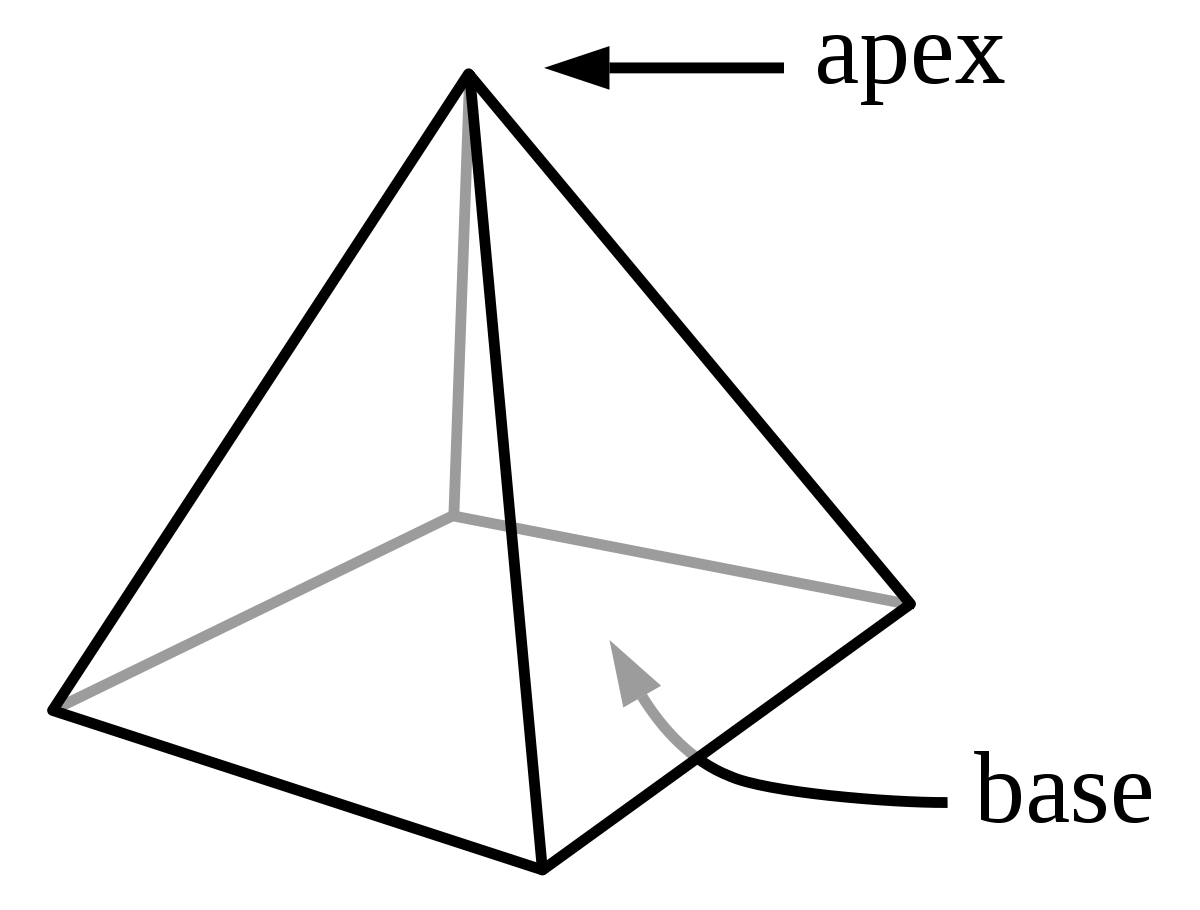
\includegraphics[width=0.2\textwidth]{imgs/pyramide.png}
\end{figure}

The vertex at the apex of a pyramid has four tight constraints, but lies in 
three dimensions. This is a geometric artifact, and it is the worst case for a
simplex.\\

(ii)\\
\begin{figure}[!h]
  \label{fig:projection}
  \centering
    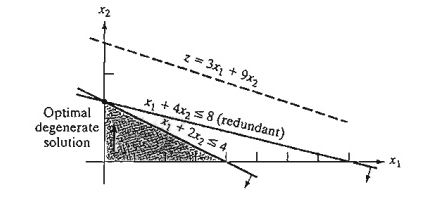
\includegraphics[width=0.5\textwidth]{imgs/triangle-degeneracy.png}
\end{figure}

In a triangle, each vertex has two tight constraints. Adding a new inequality
is redundant (do not change the polyhedron). This is a redundant artifact, and
it is easy to get rid off in the simplex.\\

\emph{Note: In dimension 2, degeneracy $\iff$ redundant. Geometric artifacts
starts at dimension 3.}\\

\emph{A constraint $A_k x \leq b_k$ is redundant if $\{ x\in \mathbb{R}^n \mid
Ax \leq b \} = \{x \in \mathbb{R}^n \mid A_1 x \leq b_1, \dots, A_{k-1} x \leq
b_{k-1}, A_{k+1} x \leq b_{k+1}, \dots, A_m x \leq b_m \}$.}\\

(iii)\\
$\{x \in \mathbb{R}^3 \mid 
\begin{bmatrix}
1 & -1 & 0\\
1 & 1 & 1
\end{bmatrix}
x =
\begin{bmatrix}
0\\
2
\end{bmatrix}$, $x \geq 0 \}$\\

BFS:
$\begin{pmatrix}
1\\
1\\
0
\end{pmatrix}$ for $B = \{1, 2\}$ or
$\begin{pmatrix}
0\\
0\\
2
\end{pmatrix}$ for $B = \{1,3\}, \{2, 3\}$

\paragraph{Theorem: Let $x^*$, $y^*$ as defined previously, $x^*$ is feasible,
then:}
\begin{enumerate}
\item if $\bar{c} \geq 0 \rightarrow x^*$ is optimal.
\item if $x^*$ is optimal and non degenerated $\rightarrow \bar{c} \geq 0$
\item if $y^*$ is feasible for the dual and $A^{-1}_B b \geq 0$ then $y^*$ is
optimal

\end{enumerate}

\subparagraph{Proof:}
\begin{enumerate}
\item Show that for any other point, the objective value is worst.\\
Let $z \in \mathcal{P}$, $d = z -x^* \rightarrow Ad = 0$.\\
Write $Ad = A_B d_B + A_N d_N$. Now, $Ad = 0 \iff d_B = -A^{-1}_B A_N d_N$.\\
Consider $c^T d = c^T_B d_B + c^T_N d_N = c^T_N d_N - c^T_B A^{-1}_B A_N d_N =
\sum_{j \in N} (c_j - c^T_B A^{-1}_B A_{\cdot j})d_j = \sum_{j \in N}
\bar{c_j}d_j$.\\
As $z \in \mathcal{P} \rightarrow \forall j \in N$, $z_j =
\underbrace{x^*_j}_{=0} + d_j \geq 0 \rightarrow d_N \geq 0$.\\
But then, $c^T z = c^T x^* + c^T d = c^T x^* +
\sum_{j \in N} \underbrace{\bar{c_j}}_{\geq 0} \underbrace{d_j}_{\geq 0}
\geq c^T x^*$. So, $c^T x^*$ is, indeed, minimal.

\item Let $x^*$ be non-degenerate $\rightarrow x^*_i > 0$, $\forall i \in B$.
Assume that $\exists j \in N$: $\bar{c_j} < 0$ and $x^*$ is optimal.\\
Let $d =
\begin{pmatrix}
d_B\\
d_N
\end{pmatrix}
=
\begin{pmatrix}
-A^{-1}_B A_{\cdot j}\\
\underbrace{e_j}_{(0,\dots, 0, 1, 0, \dots) \in \mathbb{Z}^{|N|}}
\end{pmatrix}$.
Now, $\exists \epsilon > 0$ st $x^* + \epsilon d \in \mathcal{P}$.\\
$Ad = -\underbrace{A_B A^{-1}_B}_{Im} + \underbrace{A_N e_j}_{A_{\cdot j}} =
0$.\\
As $x^*_i > 0$, $\forall i \in B$, $x^*_i + \epsilon d_i \geq 0$.
Now, $c^T(x^* + \epsilon d) = c^T x^* + \epsilon c^T d = c^T x^* + \epsilon
\bar{c_j} \underbrace{d_j}_{=1} = c^T x^* + \epsilon
\underbrace{\bar{c_j}}_{< 0} < c^T x^*$.\\
So, by contradiction, no other point improves objective value of $x^*$.

\item Let $z \in \mathcal{D}$ feasible for the dual. \\
By definition, $z^T A \leq c^T \rightarrow z^T A_B \leq c^T_B$.
Now, $(y^*)^T b = c^T_B \underbrace{A^{-1}_B b}_{\geq 0}
\geq z^T A_B A^{-1}_B b = z^T b$. So, $y^*$ is optimal.

\end{enumerate}

\end{document}
